\newpage
\section{Durchführung}
\label{sec:Durchfuehrung}
\subsection{Versuchsaufbau}
Mit dem hier genutzten Aufbau lassen sich Halbwertszeiten im Bereich von Sekunden bis Stunden messen.
\begin{figure}
    \centering
    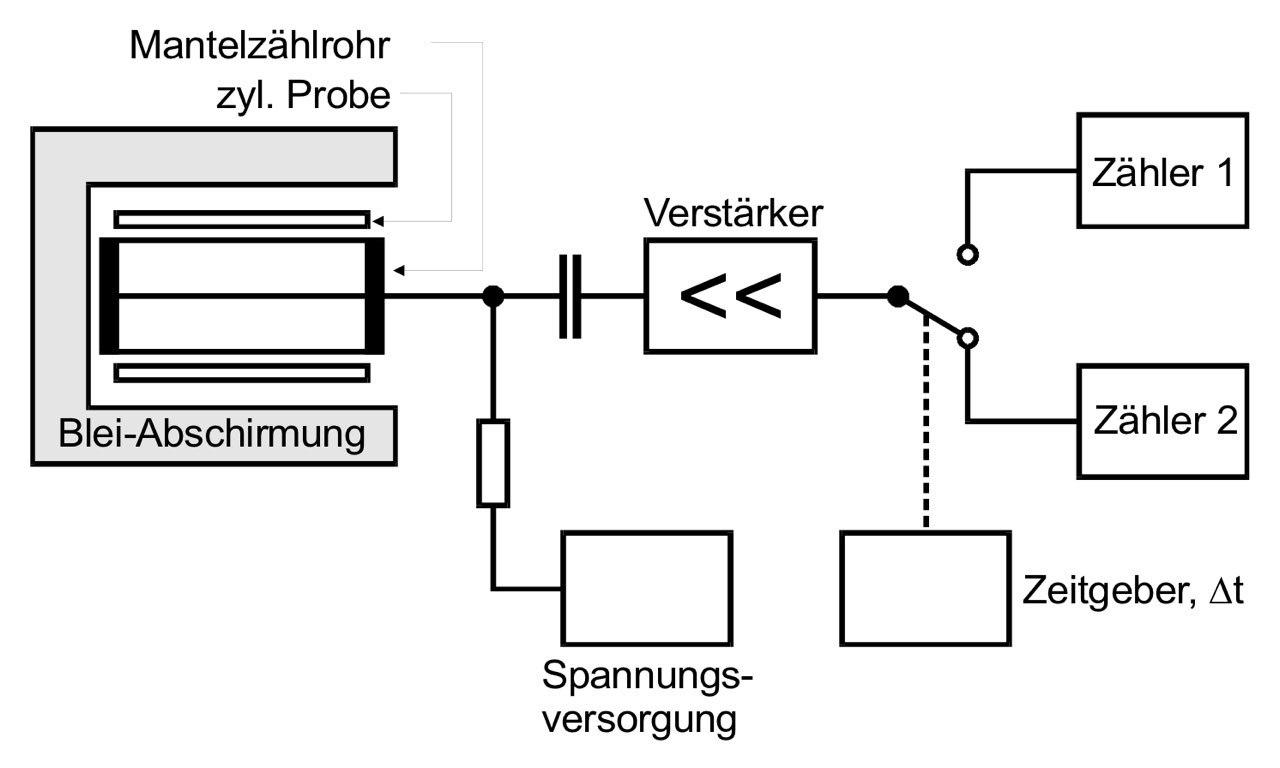
\includegraphics[width=0.7\textwidth]{bilder/Versuchsaufbau.jpg}
    \caption{Darstellung des Versuchsaufbaus.\\
    Gezeigt ist Quelle der Neutronen mit den zylindrischen Proben, abgeschirmt durch einen Bleimantel,
    der die Hintergrundstrahlung absorbieren soll.\cite[217]{anleitung}}
\end{figure}

MIthilfe eines Geiger-Müller-Zählrohres kann nun die von den zylinderförmigen Proben ausgesante $\beta-$ und 
$\gamma-$Strahlung dedektiert werden. Um den Nulleffekt zu verringern (Einfluss der natürlichen Hintergrundstrahlung),
befindet sich das Zählrohr in eimem Abschirmblock aus Blei.
Die Messzeit $\Delta t$ lässt isch über das Gerät einstellen (rel. Genauigkeit $10^{-5}$).
\subsection{Die Zerfälle}
Untersucht werden die Zerfälle der instabilen Isotopen Rhodium $^{103}$Rh und Vanadium $^{51}$V.
\begin{align}
    \isotope[51][23]{V} + \text{n} &\to \isotope[52][23]{V} \to \isotope[52][24]{Cr} + \beta^- + \bar{\nu_{\text{e}}}\\
    \isotope[103][45]{Rh}+n&
    \begin{cases}
        \to \isotope[104\text{i}][45]Rh \to \isotope[104][45]Rh+\gamma \to \isotope[104][46]Pb+\beta^- + \bar{\nu_{\text{e}}} & 10\%\\\\
        \to \isotope[104][45]Rh \to \isotope[104][46]Pb+\beta^- + \bar{\nu_{\text{e}}} & 90\%
    \end{cases}
    \label{eqn:rh}
\end{align}
Mit dem Verfahren aus Abschnitt \ref{subsec:halbwertszeit} kann für Vanadium die Halbwertszeit ermittelt werden.
Bei Rhodium treten allerdings Besonderheiten auf.\\
So zeigt sich in der Gl. \ref{eqn:rh}, dass neben dem zu 90\% entshende instabile Isotop $^{104}$Rh ebenfalls
auch das instabile $^{104\text{i}}$Rh entstehen kann. Diese beiden Zerfälle laufen mit verschieden Halbwertszeiten $T$ 
nebeneinander ab. Der Strahlungsdetektor kann die energiearme $\gamma-$Strahlung der $^{104\text{i}}$Rh nachweisen,
sodass mit der Methodik aus Abschnitt \ref{subsec:halbwertszeit} für beide Prozesse 
die Halbwertszeit bestimmt werden kann.